% answers.tex —— 1988 年·上海卷 · 参考答案与详细解析片段
% 由 tools/generate_projects.py 依来源总账自 1988/1988_数学真题_上海_试题.md + 1988/1988_数学真题_上海_解析正文.md + 1988/1988_数学真题_上海_答案要点.md 生成，勿手改（改源 MD 后重跑）


\begin{gktip}
固定源 PDF 第 3—6 页含答案与解答。第 2 大题第 6 小题在当前扫描中缺少 A、B、C、D 四个选项，保留固定答案表代号 B，并由题干独立复算其数值。
\end{gktip}

\begin{answer}
\gksolhead{1}{}

\textbf{题目}：

一、（本题满分 30 分）本题共有 10 个小题，只要求直接填写结果。每个空格填对得 3 分，否则一律得零分。

\Needspace{5\baselineskip}
（1） 方程

\nopagebreak[4]
\[
4^x-2^{x+1}-8=0
\]

的解是　　　　。

\Needspace{5\baselineskip}
（2）　

\nopagebreak[4]
\[
y=\sqrt{x-1}
\]

的反函数是　　　　。

（3） 在极坐标系中，以 $\left(\dfrac a2,\dfrac\pi2\right)$ 为圆心、$\dfrac a2$ 为半径的圆的方程为　　　　。

\Needspace{5\baselineskip}
（4） 参数方程

\nopagebreak[4]
\[
\begin{cases}
x=1-2t,\\
y=2t^2-t
\end{cases}
\qquad(t\in\mathbb R)
\]

化为普通方程为　　　　。

（5） 一圆锥的侧面展开图是圆心角为 $216^\circ$ 的扇形，则此圆锥的轴截面的半顶角的正弦是　　　　。

\Needspace{5\baselineskip}
（6）　

\nopagebreak[4]
\[
\lim_{n\to\infty}
\frac{(-2)^{n+1}}{1-2+4-\cdots+(-2)^{n-1}}
\]

的值是　　　　。

\Needspace{5\baselineskip}
（7） 函数

\nopagebreak[4]
\[
y=\cos\left(\frac\pi2x\right)\cos\left[\frac\pi2(x-1)\right]
\]

的最小正周期是　　　　。

（8） 在 $(1+x)^n$ 的展开式中，若第三项和第六项的系数相等，则 $n=$　　　　。

\Needspace{5\baselineskip}
（9） 到椭圆

\nopagebreak[4]
\[
\frac{x^2}{25}+\frac{y^2}{9}=1
\]

右焦点的距离与直线 $x=6$ 的距离相等的动点轨迹方程是　　　　。

（10） 从 6 个运动员中选出 4 人参加 $4\times100$ 米接力赛，如果甲、乙两人都不能跑第一棒，那么共有　　　　种不同的参赛方案（要求结果用数字表示）。

\Needspace{4\baselineskip}
\textbf{解析}

\gksubpart{（1）}

\Needspace{5\baselineskip}
令 $t=2^x>0$，则

\nopagebreak[4]
\[
4^x-2^{x+1}-8=t^2-2t-8=(t-4)(t+2)=0.
\]

因此 $t=4$，即 $x=2$。

\gksubpart{（2）}

\Needspace{5\baselineskip}
由 $y=\sqrt{x-1}$ 得 $x=y^2+1$。原函数的值域为 $y\ge0$，所以反函数为

\nopagebreak[4]
\[
y=x^2+1,\qquad x\ge0.
\]

\gksubpart{（3）}

\Needspace{5\baselineskip}
极点到圆心的距离为 $a/2$，圆半径也为 $a/2$。由极坐标圆的标准关系，圆过极点且圆心在极轴正方向的夹角为 $\pi/2$，故

\nopagebreak[4]
\[
\rho=2\cdot\frac a2\sin\theta=a\sin\theta.
\]

\gksubpart{（4）}

\Needspace{5\baselineskip}
由 $x=1-2t$ 得 $t=(1-x)/2$。代入 $y=2t^2-t$：

\nopagebreak[4]
\[
y=2\left(\frac{1-x}{2}\right)^2-\frac{1-x}{2}
=\frac{x^2-x}{2}.
\]

\gksubpart{（5）}

\Needspace{5\baselineskip}
设圆锥母线长为 $l$、底面半径为 $R$，则侧面展开扇形的弧长满足

\nopagebreak[4]
\[
\frac{216^\circ}{360^\circ}\cdot2\pi l=2\pi R,
\qquad\text{\text{所以}}\qquad \frac Rl=\frac35.
\]

\Needspace{5\baselineskip}
轴截面半顶角为 $\varphi$ 时 $\sin\varphi=R/l$，故

\nopagebreak[4]
\[
\sin\varphi=\frac35.
\]

\gksubpart{（6）}

\Needspace{5\baselineskip}
分母是等比数列前 $n$ 项和：

\nopagebreak[4]
\[
1-2+4-\cdots+(-2)^{n-1}
=\frac{1-(-2)^n}{3}.
\]

\Needspace{5\baselineskip}
因此

\nopagebreak[4]
\[
\lim_{n\to\infty}
\frac{(-2)^{n+1}}{(1-(-2)^n)/3}
=6.
\]

\gksubpart{（7）}

\Needspace{5\baselineskip}
积化和差得

\nopagebreak[4]
\[
\begin{aligned}
y
&=\frac12\left[
\cos\left(\frac\pi2\right)
+\cos\left(\pi x-\frac\pi2\right)\right]\\
&=\frac12\sin\pi x.
\end{aligned}
\]

所以最小正周期为 $2$。

\gksubpart{（8）}

\Needspace{5\baselineskip}
第三项和第六项的系数分别为 $\binom n2$ 和 $\binom n5$。由

\nopagebreak[4]
\[
\binom n2=\binom n5
\]

得 $n-2=5$，即 $n=7$。

\gksubpart{（9）}

\Needspace{5\baselineskip}
椭圆

\nopagebreak[4]
\[
\frac{x^2}{25}+\frac{y^2}{9}=1
\]

\Needspace{5\baselineskip}
的右焦点为 $(4,0)$。由动点到焦点和直线 $x=6$ 的距离相等：

\nopagebreak[4]
\[
\sqrt{(x-4)^2+y^2}=|x-6|.
\]

\Needspace{5\baselineskip}
平方整理得

\nopagebreak[4]
\[
y^2=-4(x-5).
\]

\gksubpart{（10）}

\Needspace{5\baselineskip}
第一棒可从不能跑第一棒的甲、乙之外的 4 人中选出；其余三棒从剩下的 5 人中依次安排。因此方案数为

\nopagebreak[4]
\[
4\cdot5\cdot4\cdot3=240.
\]

\gkanswer{答案（1）：$2$}

\gkanswer{答案（2）：$y=x^2+1\ (x\ge0)$}

\gkanswer{答案（3）：$\rho=a\sin\theta$}

\gkanswer{答案（4）：$y=\dfrac{x^2-x}{2}$}

\gkanswer{答案（5）：$\dfrac35$}

\gkanswer{答案（6）：$6$}

\gkanswer{答案（7）：$2$}

\gkanswer{答案（8）：$7$}

\gkanswer{答案（9）：$y^2=-4(x-5)$}

\gkanswer{答案（10）：$240$}

\end{answer}
\begin{answer}
\gksolhead{2}{}

\textbf{题目}：

二、（本题满分 30 分）本题共有 10 个小题，每一个小题都给出代号为 A、B、C、D 的四个结论，其中有且只有一个结论是正确的，必须把正确结论的代号写在题后的圆括号内。选对得 3 分，不选、选错或选出的代号超过一个（不论是否都写在圆括号内），一律得零分。

\Needspace{5\baselineskip}
（1） 方程

\nopagebreak[4]
\[
x^4-y^4-4x^2+4y^2=0
\]

所表示的曲线是\mbox{（　　）}

（A）双曲线和一个圆　　（B）两条相交直线

（C）两条平行直线和一个圆　　（D）两条相交直线和一个圆

（2） 在 $\left[-1,\dfrac32\right]$ 上与函数 $y=x$ 相同的函数是\mbox{（　　）}

（A）$y=\arccos(\cos x)$　　（B）$y=\arcsin(\sin x)$

（C）$y=\sin(\arcsin x)$　　（D）$y=\cos(\arccos x)$

\Needspace{5\baselineskip}
（3） 函数

\nopagebreak[4]
\[
y=\frac{1+a^x}{1-a^x}\qquad(a>0,\ a\ne1)
\]

（A）是奇函数　　（B）是偶函数

（C）既是奇函数，又是偶函数　　（D）是非奇非偶函数

（4） $|x|\le2$ 是 $|x+1|<1$ 的\mbox{（　　）}

（A）必要不充分条件　　（B）充分不必要条件

（C）充分必要条件　　（D）既不充分也不必要条件

（5） 下列命题中错误的是\mbox{（　　）}

（A）若一直线垂直于一平面，则此直线必垂直于这平面上所有直线；

（B）若一个平面通过另一个平面的一条垂线，则这两个平面互相垂直；

（C）若一直线垂直于一个平面的一条垂线，则此直线平行于这个平面；

（D）若平面内的一条直线和这个平面的一条斜线的射影垂直，则它也和这条斜线垂直。

（6） 若 $\sin\alpha=\dfrac5{13}$，$\alpha$ 为第二象限角，则 $\operatorname{tg}\dfrac\alpha2$ 的值为　　　　。

\begin{gktip}
\textbf{转录疑点}：固定源第 2 页第 6 小题只见题干，当前扫描中未见其 A、B、C、D 四个选项；固定答案表仍记录该小题答案代号为 B。
\end{gktip}

（7） 在半径为 $a$ 的球中，高为 $\dfrac23a$ 的球冠面积与整个球面面积之和为\mbox{（　　）}

（A）$\dfrac83\pi a^2$　　（B）$\dfrac{10}3\pi a^2$　　（C）$\dfrac{14}3\pi a^2$　　（D）$\dfrac{16}3\pi a^2$

（8） 下列函数图象中正确的是\mbox{（　　）}
\nopagebreak[4]
\begin{center}% 1988 年上海卷第二大题第 8 小题：四个函数图象选项示意
\begin{tikzpicture}[scale=0.72,>=stealth,font=\scriptsize]
  \begin{scope}[shift={(-3.0,2.25)}]
    \draw[->] (-1.4,0)--(1.65,0) node[right] {$x$};
    \draw[->] (0,-1.1)--(0,1.75) node[above] {$y$};
    \draw[thick] (-1.25,-0.9)--(1.25,1.35);
    \draw[thick,domain=0.08:1.45,samples=60]
      plot (\x,{0.8*ln(\x)/ln(2)});
    \node[above] at (0.7,1.48) {$y=x+a$};
    \node[right] at (1.32,0.35) {$y=\log_2x$};
    \node[below] at (0,-1.45) {（A）};
  \end{scope}
  \begin{scope}[shift={(1.0,2.25)}]
    \draw[->] (-1.4,0)--(1.65,0) node[right] {$x$};
    \draw[->] (0,-1.1)--(0,1.75) node[above] {$y$};
    \draw[thick] (-1.25,-0.9)--(1.25,1.35);
    \draw[thick,domain=-1.25:1.4,samples=80]
      plot (\x,{0.9*exp(-0.85*\x)});
    \node[above right] at (0.35,1.47) {$y=a^x$};
    \node[right] at (1.15,0.45) {$y=x+a$};
    \node[below] at (0,-1.45) {（B）};
  \end{scope}
  \begin{scope}[shift={(-3.0,-1.35)}]
    \draw[->] (-1.4,0)--(1.65,0) node[right] {$x$};
    \draw[->] (0,-1.1)--(0,1.75) node[above] {$y$};
    \draw[thick] (-1.25,-0.9)--(1.25,1.35);
    \draw[thick,domain=0:1.45,samples=70]
      plot (\x,{0.85*\x^0.55});
    \node[above right] at (0.48,1.4) {$y=x^a$};
    \node[below] at (0,-1.45) {（C）};
  \end{scope}
  \begin{scope}[shift={(1.0,-1.35)}]
    \draw[->] (-1.4,0)--(1.65,0) node[right] {$x$};
    \draw[->] (0,-1.1)--(0,1.75) node[above] {$y$};
    \draw[thick] (-1.25,-0.9)--(1.25,1.35);
    \draw[thick,domain=-1.25:-0.08,samples=60]
      plot (\x,{-0.55*sqrt(-\x)});
    \draw[thick,domain=0.08:1.45,samples=60]
      plot (\x,{0.55*sqrt(\x)});
    \node[right] at (0.48,0.73) {$y=x^a$};
    \node[below] at (0,-1.45) {（D）};
  \end{scope}
\end{tikzpicture}
\end{center}
\nopagebreak[4]
（9） 下列关系中正确的是\mbox{（　　）}

（A）$\left(\dfrac12\right)^{\frac23}<\left(\dfrac15\right)^{\frac23}<\left(\dfrac12\right)^{\frac13}$

（B）$\left(\dfrac12\right)^{-\frac13}<\left(\dfrac12\right)^{\frac23}<\left(\dfrac15\right)^{\frac23}$

（C）$\left(\dfrac15\right)^{-\frac23}<\left(\dfrac12\right)^{-\frac13}<\left(\dfrac12\right)^{\frac23}$

（D）$\left(\dfrac13\right)^{\frac23}<\left(\dfrac12\right)^{\frac23}<\left(\dfrac12\right)^{\frac13}$

（10） 方程 $\sin x=\lg x$ 的实数根有\mbox{（　　）}

（A）1 个　　（B）2 个　　（C）3 个　　（D）无穷多个

\Needspace{4\baselineskip}
\textbf{解析}

\gksubpart{（1）}

\nopagebreak[4]
\[
x^4-y^4-4x^2+4y^2
=(x^2-y^2)(x^2+y^2-4).
\]

故图形是两条相交直线 $x^2-y^2=0$ 与圆 $x^2+y^2=4$，选 D。

\gksubpart{（2）}

\Needspace{5\baselineskip}
因为

\nopagebreak[4]
\[
-1\ge-\frac\pi2,\qquad \frac32<\frac\pi2,
\]

所以在 $\left[-1,\dfrac32\right]$ 上 $\arcsin(\sin x)=x$，选 B。

\gksubpart{（3）}

\nopagebreak[4]
\[
f(-x)=\frac{1+a^{-x}}{1-a^{-x}}
=\frac{a^x+1}{a^x-1}
=-f(x).
\]

故 $f$ 是奇函数，选 A。

\gksubpart{（4）}

由 $|x+1|<1$ 得 $-2<x<0$，这一定包含于 $|x|\le2$ 的解集内；反之不成立。因此 $|x|\le2$ 是 $|x+1|<1$ 的必要不充分条件，选 A。

\gksubpart{（5）}

选项 C 的条件只说明该直线垂直于平面内的一条直线，不能推出它平行于这个平面，因此错误命题为 C。

\gksubpart{（6）}

\Needspace{5\baselineskip}
由 $\sin\alpha=5/13$ 且 $\alpha$ 在第二象限，得 $\cos\alpha=-12/13$。于是

\nopagebreak[4]
\[
\operatorname{tg}\frac\alpha2
=\frac{\sin\alpha}{1+\cos\alpha}
=\frac{5/13}{1/13}=5.
\]

固定源该小题的四个选项缺失，但答案表记录的代号为 B。

\gksubpart{（7）}

\Needspace{5\baselineskip}
球冠面积为

\nopagebreak[4]
\[
S_{\text{\text{冠}}}=2\pi a\cdot\frac{2a}{3}
=\frac43\pi a^2.
\]

\Needspace{5\baselineskip}
整个球面面积为 $4\pi a^2$，两者之和为

\nopagebreak[4]
\[
\frac43\pi a^2+4\pi a^2
=\frac{16}{3}\pi a^2,
\]

选 D。

\gksubpart{（8）}

逐项检查函数的定义域、单调性、截距与曲线的凹凸关系，只有图 B 同时符合图中标注的指数函数、对数函数和直线关系，选 B。

\gksubpart{（9）}

\Needspace{5\baselineskip}
选项 D 中

\nopagebreak[4]
\[
\left(\frac13\right)^{2/3}
<\left(\frac12\right)^{2/3}
<\left(\frac12\right)^{1/3},
\]

因为底数均在 $(0,1)$ 内，且相同底数的指数越大，幂越小；又 $1/3<1/2$。故选 D。

\gksubpart{（10）}

\Needspace{5\baselineskip}
比较 $\sin x$ 与 $\lg x$ 在各个单调区间的符号和端点值，可知在

\nopagebreak[4]
\[
\left(\frac\pi2,\pi\right),\qquad
\left(2\pi,\frac{5\pi}{2}\right),\qquad
\left(\frac{5\pi}{2},3\pi\right)
\]

各有一个交点，其他区间无交点，故共有 3 个实数根，选 C。

\gkanswer{答案（1）：D}

\gkanswer{答案（2）：B}

\gkanswer{答案（3）：A}

\gkanswer{答案（4）：A}

\gkanswer{答案（5）：C}

\gkanswer{答案（6）：B（固定源选项缺失；由题干可复算 $\operatorname{tg}(\alpha/2)=5$）}

\gkanswer{答案（7）：D}

\gkanswer{答案（8）：B}

\gkanswer{答案（9）：D}

\gkanswer{答案（10）：C}

\end{answer}
\begin{answer}
\gksolhead{3}{}

\textbf{题目}：

三、（本题满分 30 分）本题共有 4 个小题，第 1、2 小题等题满分 7 分，第 3、4 小题等题满分 8 分。

\Needspace{5\baselineskip}
（1） 已知直线

\nopagebreak[4]
\[
l_1:3x-y+12=0,\qquad l_2:3x+2y-6=0.
\]

求 $l_1$、$l_2$ 和 $y$ 轴所围成的三角形面积。

\Needspace{5\baselineskip}
（2） 设

\nopagebreak[4]
\[
A=\left\{x\mathrel{}\middle|\mathrel{}x\ge\frac1x,\ x\in\mathbb R\right\},
\qquad
B=\left\{x\mathrel{}\middle|\mathrel{}\sqrt{2x+1}<3,\ x\in\mathbb R\right\}.
\]

求 $D=A\cap B$。

（3） 一个圆锥容器和一个圆柱形容器，它们的轴截面尺寸如图。两容器内盛有的液体的体积正好相等，且液面高度 $h$ 正好相同。求 $h$。
\nopagebreak[4]
\begin{center}% 1988 年上海卷第三题：圆锥、圆柱轴截面示意图
\begin{tikzpicture}[scale=0.7,>=stealth,font=\small]
  \begin{scope}[shift={(-3.0,0)}]
    \coordinate (L) at (-1.55,1.25);
    \coordinate (R) at (1.55,1.25);
    \coordinate (V) at (0,-1.25);
    \draw[thick] (L)--(V)--(R)--cycle;
    \draw[dashed] (0,1.25)--(V);
    \draw[thin] (-1.55,0.25)--(1.55,0.25);
    \draw[<->] (-1.55,1.52)--(0,1.52)
      node[midway,above] {$a$};
    \draw[<->] (-1.85,1.25)--(-1.85,-1.25)
      node[midway,left] {$a$};
    \draw[<->] (1.85,0.25)--(1.85,-1.25)
      node[midway,right] {$h$};
    \node[below] at (0,-1.65) {圆锥};
  \end{scope}
  \begin{scope}[shift={(2.1,0)}]
    \draw[thick] (-1.0,-1.25)--(-1.0,1.25)--(1.0,1.25)--(1.0,-1.25)--cycle;
    \draw[dashed] (0,-1.45)--(0,1.45);
    \draw[thin] (-1.0,0.25)--(1.0,0.25);
    \draw[<->] (-1.0,1.52)--(0,1.52)
      node[midway,above] {$\dfrac a2$};
    \draw[<->] (1.3,0.25)--(1.3,-1.25)
      node[midway,right] {$h$};
    \node[below] at (0,-1.65) {圆柱};
  \end{scope}
\end{tikzpicture}
\end{center}
\nopagebreak[4]
\Needspace{5\baselineskip}
（4） 设方程

\nopagebreak[4]
\[
x^2+3\sqrt3x+4=0
\]

\Needspace{5\baselineskip}
的两个实根为 $x_1\text{、}x_2$。记

\nopagebreak[4]
\[
\alpha=\arctan x_1,\qquad \beta=\arctan x_2.
\]

求 $\alpha+\beta$。

\Needspace{4\baselineskip}
\textbf{解析}

\gksubpart{（1）}

\Needspace{5\baselineskip}
直线 $l_1$、$l_2$ 在 $y$ 轴上的截距分别为 $12$ 和 $3$，所以它们在 $y$ 轴上截出的底边长为 $9$。由两直线联立可得交点横坐标为 $-2$，交点到 $y$ 轴的距离为 $2$。因此三角形面积为

\nopagebreak[4]
\[
S=\frac12\cdot9\cdot2=9.
\]

\gksubpart{（2）}

\Needspace{5\baselineskip}
对集合 $A$ 分 $x>0$ 和 $x<0$ 讨论：

\nopagebreak[4]
\[
x\ge\frac1x
\quad\Longleftrightarrow\quad
A=[-1,0)\cup[1,+\infty).
\]

\Needspace{5\baselineskip}
而

\nopagebreak[4]
\[
\sqrt{2x+1}<3
\quad\Longleftrightarrow\quad
-\frac12\le x<4,
\]

\Needspace{5\baselineskip}
所以

\nopagebreak[4]
\[
D=A\cap B=[-1,0)\cup[1,4).
\]

\gksubpart{（3）}

\Needspace{5\baselineskip}
由图，圆锥容器的轴截面底角为 $45^\circ$，且圆锥与圆柱的液面高度相同为 $h$。因此圆锥内液面半径为 $h$，其液体体积为

\nopagebreak[4]
\[
V_{\text{\text{锥}}}=\frac13\pi h^2h=\frac\pi3h^3.
\]

\Needspace{5\baselineskip}
圆柱容器半径为 $a/2$，液体体积为

\nopagebreak[4]
\[
V_{\text{\text{柱}}}=\pi\left(\frac a2\right)^2h=\frac{\pi a^2h}{4}.
\]

\Needspace{5\baselineskip}
体积相等且 $h>0$，故

\nopagebreak[4]
\[
\frac\pi3h^3=\frac{\pi a^2h}{4}
\quad\Longrightarrow\quad
h=\frac{\sqrt3}{2}a.
\]

\gksubpart{（4）}

\Needspace{5\baselineskip}
由韦达定理

\nopagebreak[4]
\[
x_1+x_2=-3\sqrt3,\qquad x_1x_2=4.
\]

\Needspace{5\baselineskip}
于是

\nopagebreak[4]
\[
\tan(\alpha+\beta)
=\frac{x_1+x_2}{1-x_1x_2}
=\frac{-3\sqrt3}{-3}
=\sqrt3.
\]

\Needspace{5\baselineskip}
又 $x_1,x_2<0$，所以 $\alpha,\beta\in(-\pi/2,0)$，从而 $\alpha+\beta\in(-\pi,0)$。因此

\nopagebreak[4]
\[
\alpha+\beta=-\frac{2\pi}{3}.
\]

\gkanswer{答案（1）：$9$}

\gkanswer{答案（2）：$\left[-1,0\right)\cup\left[1,4\right)$}

\gkanswer{答案（3）：$h=\dfrac{\sqrt3}{2}a$}

\gkanswer{答案（4）：$\alpha+\beta=-\dfrac{2\pi}{3}$}

\end{answer}
\begin{answer}
\gksolhead{4}{}

\textbf{题目}：

\Needspace{5\baselineskip}
四、（本题满分 15 分）设 $a>0$，$b>0$，

\nopagebreak[4]
\[
y=\log_{\frac12}\left[a^{2x}+2(ab)^x-b^{2x}+1\right].
\]

求使 $y$ 为负值的 $x$ 的取值范围。

\Needspace{4\baselineskip}
\textbf{解析}

\Needspace{5\baselineskip}
因底数 $1/2$ 小于 $1$，$y<0$ 等价于真数大于 $1$：

\nopagebreak[4]
\[
a^{2x}+2(ab)^x-b^{2x}>0.
\]

\Needspace{5\baselineskip}
提取 $b^{2x}>0$，令 $t=(a/b)^x$，得

\nopagebreak[4]
\[
t^2+2t-1>0.
\]

\Needspace{5\baselineskip}
因 $t>0$，所以

\nopagebreak[4]
\[
t>\sqrt2-1.
\]

\Needspace{5\baselineskip}
分情况讨论：

\nopagebreak[4]
\[
\begin{cases}
x>\log_{a/b}(\sqrt2-1),&a>b>0,\\
x<\log_{a/b}(\sqrt2-1),&0<a<b,\\
x\in\mathbb R,&a=b>0.
\end{cases}
\]

\gkanswer{答案：当 $a>b>0$ 时，$x>\log_{\frac ab}(\sqrt2-1)$；当 $0<a<b$ 时，$x<\log_{\frac ab}(\sqrt2-1)$；当 $a=b>0$ 时，$x\in\mathbb R$。}

\end{answer}
\begin{answer}
\gksolhead{5}{}

\textbf{题目}：

五、（本题满分 15 分）本题共有 2 个小题，第 1 小题满分 7 分，第 2 小题满分 8 分。

在棱长都相等的四面体 $A-BCD$ 中，$E\text{、}F$ 分别为棱 $AD\text{、}BC$ 的中点，连接 $AF\text{、}CE$，如图所示。
\nopagebreak[4]
\begin{center}% 1988 年上海卷第五题：正四面体 A-BCD，E/F 为中点
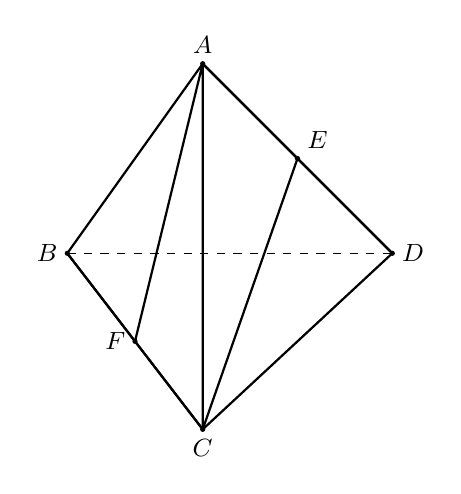
\begin{tikzpicture}[scale=0.86,>=stealth,font=\small]
  \coordinate (A) at (0,3.8);
  \coordinate (B) at (-2.0,1.0);
  \coordinate (C) at (0,-1.6);
  \coordinate (D) at (2.8,1.0);
  \coordinate (E) at (1.4,2.4);
  \coordinate (F) at (-1.0,-0.3);
  \draw[thick] (A)--(B)--(C)--(D)--cycle;
  \draw[thick] (A)--(C) (A)--(F) (C)--(E);
  \draw[dashed] (B)--(D);
  \draw[thick] (B)--(F)--(C);
  \draw[thick] (A)--(E)--(D);
  \fill (A) circle (1.1pt) node[above] {$A$};
  \fill (B) circle (1.1pt) node[left] {$B$};
  \fill (C) circle (1.1pt) node[below] {$C$};
  \fill (D) circle (1.1pt) node[right] {$D$};
  \fill (E) circle (1.1pt) node[above right] {$E$};
  \fill (F) circle (1.1pt) node[left] {$F$};
\end{tikzpicture}
\end{center}
\nopagebreak[4]
（1） 求异面直线 $AF\text{、}CE$ 所成角的大小。

（2） 求 $CE$ 与底面 $BCD$ 所成角的大小（要求角的大小用反三角函数表示）。

\Needspace{4\baselineskip}
\textbf{解析}

设四面体棱长为 $a$。取 $DF$ 的中点为 $G$，连接 $GE$、$GC$。

\gksubpart{（1）}

\Needspace{5\baselineskip}
在三角形 $AFD$ 中，$E$、$G$ 分别是 $AD$、$DF$ 的中点，所以

\nopagebreak[4]
\[
EG\parallel AF,\qquad EG=\frac12AF=\frac{\sqrt3}{4}a.
\]

\Needspace{5\baselineskip}
由正四面体的等边三角形关系，

\nopagebreak[4]
\[
AF=CE=\frac{\sqrt3}{2}a,\qquad
GC=\sqrt{FC^2+FG^2}=\frac{\sqrt7}{4}a.
\]

\Needspace{5\baselineskip}
因此在三角形 $GEC$ 中

\nopagebreak[4]
\[
\cos\angle GEC
=\frac{EG^2+CE^2-GC^2}{2EG\cdot CE}
=\frac23.
\]

\Needspace{5\baselineskip}
又 $EG\parallel AF$，所以异面直线 $AF\text{、}CE$ 所成的角为

\nopagebreak[4]
\[
\arccos\frac23.
\]

\gksubpart{（2）}

过 $E$ 作 $EK\perp DF$，连接 $KC$。因 $AF\perp BC$、$DF\perp BC$，所以 $BC\perp$ 平面 $ADF$，从而 $EK\perp$ 平面 $BCD$。故 $\angle KCE$ 是 $CE$ 与底面 $BCD$ 所成的角。

\Needspace{5\baselineskip}
在三角形 $AFD$ 中，

\nopagebreak[4]
\[
EF=\sqrt{FD^2-ED^2}=\frac{\sqrt2}{2}a.
\]

\Needspace{5\baselineskip}
由相似三角形关系

\nopagebreak[4]
\[
EK=\frac{EF\cdot ED}{FD}=\frac{\sqrt6}{6}a.
\]

\Needspace{5\baselineskip}
于是

\nopagebreak[4]
\[
\sin\angle KCE=\frac{EK}{CE}
=\frac{\sqrt6\,a/6}{\sqrt3\,a/2}
=\frac{\sqrt2}{3}.
\]

\Needspace{5\baselineskip}
所以所求角为

\nopagebreak[4]
\[
\arcsin\frac{\sqrt2}{3}.
\]

\gkanswer{答案（1）：$\arccos\dfrac23$}

\gkanswer{答案（2）：$\arcsin\dfrac{\sqrt2}{3}$}

\end{answer}
\begin{answer}
\gksolhead{6}{}

\textbf{题目}：

\Needspace{5\baselineskip}
六、（本题满分 15 分）复数 $z_1\text{、}z_2\text{、}z_3$ 的辐角分别为 $\alpha\text{、}\beta\text{、}\gamma$，又

\nopagebreak[4]
\[
|z_1|=1,\qquad |z_2|=k,\qquad |z_3|=2-k,
\]

\Needspace{5\baselineskip}
且

\nopagebreak[4]
\[
z_1+z_2+z_3=0.
\]

问 $k$ 各为何值时，$\cos(\beta-\gamma)$ 分别取最大值和最小值，并求出最大值和最小值。

\Needspace{4\baselineskip}
\textbf{解析}

\Needspace{5\baselineskip}
由 $z_1+z_2+z_3=0$，三个向量的长度 $1\text{、}k\text{、}2-k$ 能组成三角形。令 $\delta=\beta-\gamma$，则

\nopagebreak[4]
\[
1=|z_2+z_3|^2
=k^2+(2-k)^2+2k(2-k)\cos\delta.
\]

\Needspace{5\baselineskip}
所以

\nopagebreak[4]
\[
\cos(\beta-\gamma)
=\frac{-2k^2+4k-3}{2k(2-k)}
=1+\frac{3}{2(k-1)^2-2}.
\]

\Needspace{5\baselineskip}
三角形条件给出

\nopagebreak[4]
\[
\frac12\le k\le\frac32.
\]

\Needspace{5\baselineskip}
在此区间内，函数在 $k=1$ 时取得最大值：

\nopagebreak[4]
\[
\cos(\beta-\gamma)_{\max}=-\frac12.
\]

\Needspace{5\baselineskip}
当 $k=\dfrac12$ 或 $k=\dfrac32$ 时，三角形退化，取得最小值

\nopagebreak[4]
\[
\cos(\beta-\gamma)_{\min}=-1.
\]

\gkanswer{答案：当 $k=1$ 时，$\cos(\beta-\gamma)$ 取得最大值 $-\dfrac12$；当 $k=\dfrac12$ 或 $k=\dfrac32$ 时，取得最小值 $-1$。}

\end{answer}
\begin{answer}
\gksolhead{7}{}

\textbf{题目}：

七、（本题满分 15 分）本题共有 2 个小题，第 1 小题满分 5 分，第 2 小题满分 10 分。

\Needspace{5\baselineskip}
在双曲线

\nopagebreak[4]
\[
\frac{y^2}{12}-\frac{x^2}{13}=1
\]

的一支上不同的三点 $A(x_1,y_1)$、$B(\sqrt{26},6)$、$C(x_2,y_2)$ 与焦点 $F(0,5)$ 的距离成等差数列。

（1） 求 $y_1+y_2$。

（2） 证明线段 $AC$ 的垂直平分线经过某一定点，并求该定点的坐标。

\begin{gktip}
题面署名：上海市四平中学　马积祥提供。
\end{gktip}

\Needspace{4\baselineskip}
\textbf{解析}

\Needspace{5\baselineskip}
双曲线的半实轴、半虚轴和半焦距分别为

\nopagebreak[4]
\[
a_0=2\sqrt3,\qquad b_0=\sqrt{13},\qquad c=5.
\]

\Needspace{5\baselineskip}
上支焦点为 $F(0,5)$。对上支任一点 $P(x,y)$，由双曲线定义或平方差关系可得

\nopagebreak[4]
\[
|PF|=\frac ca\,y-a
=\frac{5}{2\sqrt3}y-2\sqrt3.
\]

\Needspace{5\baselineskip}
点 $B(\sqrt{26},6)$ 到 $F$ 的距离为

\nopagebreak[4]
\[
|BF|=\sqrt{26+(6-5)^2}=3\sqrt3.
\]

\gksubpart{（1）}

\Needspace{5\baselineskip}
由于 $A\text{、}B\text{、}C$ 到 $F$ 的距离成等差数列，$B$ 项居中，所以

\nopagebreak[4]
\[
|AF|+|CF|=2|BF|=6\sqrt3.
\]

\Needspace{5\baselineskip}
代入上面的焦点距离表达式：

\nopagebreak[4]
\[
\frac{5}{2\sqrt3}(y_1+y_2)-4\sqrt3=6\sqrt3.
\]

\Needspace{5\baselineskip}
因此

\nopagebreak[4]
\[
y_1+y_2=12.
\]

\gksubpart{（2）}

\Needspace{5\baselineskip}
设线段 $AC$ 的垂直平分线与 $y$ 轴交于 $D(0,y_0)$。由中垂线上的等距关系，

\nopagebreak[4]
\[
x_1^2+(y_1-y_0)^2
=x_2^2+(y_2-y_0)^2.
\]

\Needspace{5\baselineskip}
整理得

\nopagebreak[4]
\[
y_0-6=\frac{x_1^2-x_2^2}{2(y_1-y_2)}.
\]

\Needspace{5\baselineskip}
又由双曲线方程

\nopagebreak[4]
\[
x_i^2=\frac{13}{12}(y_i^2-12)
\]

\Needspace{5\baselineskip}
以及第（1）问 $y_1+y_2=12$，可得

\nopagebreak[4]
\[
x_1^2-x_2^2=13(y_1-y_2).
\]

\Needspace{5\baselineskip}
所以

\nopagebreak[4]
\[
y_0-6=\frac{13}{2},
\qquad
y_0=\frac{25}{2}.
\]

\Needspace{5\baselineskip}
故垂直平分线经过定点

\nopagebreak[4]
\[
\left(0,\frac{25}{2}\right).
\]

\gkanswer{答案（1）：$y_1+y_2=12$}

\gkanswer{答案（2）：定点为 $\left(0,\dfrac{25}{2}\right)$。}

\end{answer}